\documentclass[11pt]{beamer}

\usetheme[progressbar=foot]{metropolis}
\usepackage{appendixnumberbeamer}

\usepackage{booktabs}
\usepackage[scale=2]{ccicons}

\usepackage{pgfplots}
\usepgfplotslibrary{dateplot}

\usepackage{subcaption}
\usepackage{xspace}


\newlength\mylen
\usepackage{array}
\newcolumntype{C}[1]{>{\hfil$}p{#1}<{$\hfil}}

\usepackage{adjustbox}
\usepackage{arydshln}

\definecolor{lblue}{RGB}{0, 153, 255}
\definecolor{Bg}{HTML}{f8f8f8}
\definecolor{A}{HTML}{54c9f5}%00adef}
\definecolor{B}{HTML}{625f60}%5a5758}
\definecolor{X}{HTML}{7341a0}%5f2792}
\definecolor{Kt}{HTML}{f0d757}
\definecolor{HTL}{HTML}{bd3838}
\definecolor{Per}{HTML}{cf572e}
\definecolor{ETL}{HTML}{e3e3e3}
\definecolor{An}{HTML}{e6e6b8}
\setbeamercolor{title separator}{fg=lblue}
\setbeamercolor{progress bar}{fg=lblue}
\setlength\fboxrule{2pt}

\newcommand{\blankframe}{{\setbeamercolor{background canvas}{bg=black}\frame[plain]{}}}

\title{Wavelet-Kompression und Multiskalenanalyse}
\subtitle{Vortrag zum Thema `Mathematik in Computerspielen'}
% \date{\today}
\date{22. Mai 2018}
\author{Simon Cordes \& Niklas Budinger}
\institute{JGU Mainz}
% \titlegraphic{\hfill\includegraphics[height=1.5cm]{logo.pdf}}

\begin{document}
	
	\maketitle
	
	\section{Multiskalenanalyse}
	
	{\setbeamertemplate{frame footer}{Quelle}
	\begin{frame}{Titel}
		\begin{columns}[T,onlytextwidth]
			\column{0.75\textwidth}
			Inhalt
			\column{0.25\textwidth}
			Inhalt 2
		\end{columns}
		Inhalt 3 \pause
		\begin{columns}[c,onlytextwidth]
			\column{0.38\textwidth}
			\centering
			Inhalt 4
			
			\column{0.61\textwidth}
			\vspace{15pt}\ \\
			\centering {\large$\Rightarrow$ Inhalt 5}
		\end{columns}
	\end{frame}}
	\section{Algorithmen} {

\begin{frame}{Algorithmen}
\begin{center}
\begin{tabular}{ccc}
\begin{tabular}{c}Haar-Wavelet- \\ Transformation\end{tabular} & 
$\longleftrightarrow$ & 
\begin{tabular}{c}Basiswechsel zwischen \\ Orthonormalbasen\end{tabular} \\
\end{tabular}
\\[1.0cm]
\end{center}

Zwei Ansätze:
\begin{itemize}
\item einzelne Koeffizienten: Projektion durch Skalarprodukt
\item gesamte Transformation: Filterbank-Algorithmus
\end{itemize}

\end{frame}


\begin{frame}{Erinnerung: Filterbank}

Die Filterbank-Transformation:\\[-0.1cm]
\[
\begin{array}{c c c c c c c c c c c}
C^{k} & \rightarrow & C^{k-1} & \rightarrow & C^{k-2} & \rightarrow & \dots & \rightarrow & C^{1} & \rightarrow & \mathbf{C^{0}} \\
 & \searrow & & \searrow & & \searrow & & \searrow & & \searrow & \\
 & & \mathbf{D^{k-1}} & & \mathbf{D^{k-2}} & & \dots & & \mathbf{D^{1}} & & \mathbf{D^{0}} \\
\end{array}
\]
\\[0.5cm]
mit
\\[0.1cm]
\center $C^{j} \quad = \quad P^{j} \enspace C^{j-1} \quad + \quad Q^{j} \enspace D^{j-1}$
\\
bzw.
\\
$C^{j-1} \quad = \quad A^{j} \enspace C^{j} \qquad, \qquad D^{j-1} \quad = \quad B^{j} \enspace C^{j}$
\\[0.25cm]

\pause[2] \textbf{Mehrere Matrixmultiplikationen -- Teuer!?}
\end{frame}

% Hier wird darauf hingewiesen, dass P und Q im Fall der Haar-Wavelet-Trafo fast nur Nullen enthalten, die Filterbank-Schritte also schneller direkt Implementiert werden können.

\begin{frame}{1D Haar-Wavelet-Transformation}
Einzelschritt im Speicher:
\\[1.0cm]
\begin{adjustbox}{max width=\textwidth ,center}
\begin{tabular}{c}
\settowidth\mylen{$\phi_{2i+1}^{j}$}
$
\begin{array}{c C{\mylen} C{\mylen} C{1.5\mylen} C{\mylen} C{\mylen} C{1.5\mylen} C{\mylen} C{\mylen}}
&
\phi_{0}^{j} & \phi_{1}^{j} & ... & \phi_{2i}^{j} & \phi_{2i+1}^{j} & ... & \phi_{n-2}^{j} & \phi_{n-1}^{j} \\ \cline{2-9}
C \hphantom{'}:
&
\multicolumn{1}{|c}{} & 
\multicolumn{1}{c}{} & 
\multicolumn{1}{c}{} & 
\multicolumn{1}{|c|}{a} & 
\multicolumn{1}{|c|}{b} & 
\multicolumn{1}{c}{} & 
\multicolumn{1}{c}{} & 
\multicolumn{1}{c|}{}
\\ \cline{2-9}
\end{array}
$
\\[-0.3cm]

\settowidth\mylen{$\phi_{2i+1}^{j}$}
$
\begin{array}{c C{\mylen} C{\mylen} C{1.4\mylen} C{\mylen} C{\mylen} C{1.4\mylen} C{\mylen} C{\mylen}}
 & & & & & & & & \\
 \hphantom{C':} &  &  & \multicolumn{2}{c}{\swarrow} & \multicolumn{2}{c}{\searrow} &  &  \\
\end{array}
$
\\[0.5cm]

\settowidth\mylen{$\psi_{\frac{n}{2}-1}^{j-1}$}
$
\begin{array}{c C{\mylen} C{0.5\mylen} C{\mylen} C{0.5\mylen} C{\mylen} C{\mylen} C{0.5\mylen} C{\mylen} C{0.5\mylen} C{\mylen}}
&
\phi_{0}^{j-1} &
... &
\phi_{i}^{j-1} &
... &
\phi_{\frac{n}{2}-1}^{j-1} &
\psi_{0}^{j-1} &
... &
\psi_{i}^{j-1} &
... &
\psi_{\frac{n}{2}-1}^{j} \\ \cline{2-11}
C':
&
\multicolumn{1}{|c}{} & 
\multicolumn{1}{c}{} & 
\multicolumn{1}{|c|}{\frac{a+b}{\sqrt{2}}} & 
\multicolumn{1}{c}{} & 
\multicolumn{1}{c:}{} & 
\multicolumn{1}{:c}{} & 
\multicolumn{1}{c}{} & 
\multicolumn{1}{|c|}{\frac{a-b}{\sqrt{2}}} & 
\multicolumn{1}{c}{} & 
\multicolumn{1}{c|}{}
\\ \cline{2-11}
\end{array}
$
\end{tabular}
\end{adjustbox}
\end{frame}

% An dieser Stelle wir der Analyse-Schritt-Algorithmus an der Tafel aufgeschrieben.

\begin{frame}{1D Haar-Wavelet-Transformation}
\center
Gesamt-Transformation im Speicher:
\\[-0.75cm]
\[
\begin{array}{*{8}{C{0.9cm}}}
\multicolumn{8}{c}{\vdots} \\
\hline \multicolumn{8}{|c|}{C^3} \\ \hline
\multicolumn{4}{r}{\swarrow} & \multicolumn{4}{l}{\searrow}\\
\hline \multicolumn{4}{|c|}{C^2} & \multicolumn{4}{|c|}{D^2}\\ \hline
\multicolumn{2}{r}{\swarrow} & \multicolumn{2}{l}{\searrow}\\
\cline{1-4} \multicolumn{2}{|c|}{C^1} & \multicolumn{2}{|c|}{D^1}\\ \cline{1-4}
\multicolumn{1}{r}{\swarrow} & \multicolumn{1}{l}{\searrow}\\
\cline{1-2} \multicolumn{1}{|c|}{C^0} & \multicolumn{1}{|c|}{D^0}\\ \cline{1-2}
\\ \hline
 & & & & & & & \\
\hline \multicolumn{1}{|c|}{C^0} & \multicolumn{1}{|c|}{D^0} & \multicolumn{2}{|c|}{D^1} & \multicolumn{4}{|c|}{D^2}\\ \hline
\end{array}
\]

\end{frame}

\begin{frame}[fragile]{1D Haar-Wavelet-Transformation}
\begin{adjustbox}{width=0.4\textwidth, center}
$
\begin{array}{*{8}{C{0.9cm}}}
\multicolumn{8}{c}{\vdots} \\
\hline \multicolumn{8}{|c|}{C^3} \\ \hline
\multicolumn{4}{r}{\swarrow} & \multicolumn{4}{l}{\searrow}\\
\hline \multicolumn{4}{|c|}{C^2} & \multicolumn{4}{|c|}{D^2}\\ \hline
\multicolumn{2}{r}{\swarrow} & \multicolumn{2}{l}{\searrow}\\
\cline{1-4} \multicolumn{2}{|c|}{C^1} & \multicolumn{2}{|c|}{D^1}\\ \cline{1-4}
\multicolumn{1}{r}{\swarrow} & \multicolumn{1}{l}{\searrow}\\
\cline{1-2} \multicolumn{1}{|c|}{C^0} & \multicolumn{1}{|c|}{D^0}\\ \cline{1-2}
\\ \hline
 & & & & & & & \\
\hline \multicolumn{1}{|c|}{C^0} & \multicolumn{1}{|c|}{D^0} & \multicolumn{2}{|c|}{D^1} & \multicolumn{4}{|c|}{D^2}\\ \hline
\end{array}
$
\end{adjustbox}
\center
\begin{adjustbox}{minipage=0.95\linewidth, fbox}
\begin{verbatim}
def analysis(C):
    C' = copy(C)    # <-- optional
    h = C.size
    while h > 1:
        C'[0:h] = analysisStep(C'[0:h])
        h = h // 2
    return C'
\end{verbatim}
\end{adjustbox}

\end{frame}

% An dieser Stelle mache ich an der Tafel die Laufzeit-Analyse. Dann kommt die Überleitung zu 2D-Signalen

\begin{frame}{2D Haar-Wavelet-Transformationen}
\textbf{Ergebnis:} \\
Die Algorithmen aus dem 1D-Fall können zur effizienten Implementierung der Transformation im Standard- und im Nicht-Standard-Fall wiederverwendet werden.
\\[1.0cm]
\textbf{Laufzeitkomplexität} für $n \times n$-Input:
\begin{itemize}
\item Standard-Basis: \\
$4n^2 - 4n$
\item Nicht-Standard-Basis: \\
$\frac{8}{3}(n^2-1)$
\end{itemize}

\end{frame}

% Das dauert deutlich zu lange....
%\begin{frame}{2D Standard-Haar-Wavelet-Transformation}
%\begin{center}
%\textbf{2D Standard-Basis}
%\end{center}
%~\\[-1.0cm]
%Basisfunktionen sind Tensorprodukte der 1D Basisfunktionen.\\
%\[\mathbf{v} = \sum_{k,l=0}^{n-1} a_{k,l}\phi_k^j(x)\phi_l^j(y)\]
%\\[-0.1cm]
%
%Ziel:\\[0.5cm]
%
%\begin{adjustbox}{max width=\textwidth ,center}
%\begin{tabular}{c c c}
%
%$
%\begin{array}{c|c|c|c|c}
% \multicolumn{1}{c}{}& \multicolumn{1}{c}{\phi_{0}^{j}(x)} & \multicolumn{1}{c}{\phi_{1}^{j}(x)} & \multicolumn{1}{c}{\phi_{2}^{j}(x)} & ... \\ \cline{2-5}
% \phi_{0}^{j}(y) & a_{0,0} & a_{1,0} & a_{2,0} & \\ \cline{2-5}
% \phi_{1}^{j}(y) & a_{0,1} & a_{1,1} & a_{2,1} & \\ \cline{2-5}
% \phi_{2}^{j}(y) & a_{0,2} & a_{1,2} & a_{2,2} & \\ \cline{2-5}
% \vdots & & & & 
%\end{array}
%$
%&
%$\overset{?}{\rightarrow}$
%&
%$
%\begin{array}{c|c|c|c|c}
% \multicolumn{1}{c}{}& \multicolumn{1}{c}{\phi_{0}^{0}(x)} & \multicolumn{1}{c}{\psi_{0}^{0}(x)} & \multicolumn{1}{c}{\psi_{0}^{1}(x)} & ... \\ \cline{2-5}
% \phi_{0}^{0}(y) & b_{0,0} & b_{1,0} & b_{2,0} & \\ \cline{2-5}
% \psi_{0}^{0}(y) & b_{0,1} & b_{1,1} & b_{2,1} & \\ \cline{2-5}
% \psi_{0}^{1}(y) & b_{0,2} & b_{1,2} & b_{2,2} & \\ \cline{2-5}
% \vdots & & & & 
%\end{array}
%$ 
%\\
%
%\end{tabular}
%\end{adjustbox}
%\end{frame}
%
%% An dieser Stelle führe an der Tafel den Ausklammer-Trick vor...
%
%\begin{frame}{2D Standard-Haar-Wavelet-Transformation}
%Anwenden der 1D Transformation auf Zeilen und Spalten:
%\\[0.75cm]
%\begin{adjustbox}{max width=\textwidth ,center}
%\begin{tabular}{c c c}
%$
%\begin{array}{c|c|c|c|c}
% \multicolumn{1}{c}{}& \multicolumn{1}{c}{\phi_{0}^{j}(x)} & \multicolumn{1}{c}{\phi_{1}^{j}(x)} & \multicolumn{1}{c}{\phi_{2}^{j}(x)} & ... \\ \cline{2-5}
% \phi_{l}^{j}(y)  & a_{0,l} & a_{1,l} & a_{2,l} & \\ \cline{2-5}
%\end{array}
%$
%&
%$\begin{array}{c}
%\\ \overset{1D}{\longleftrightarrow} \\
%\end{array}$
%&
%$
%\begin{array}{c|c|c|c|c}
% \multicolumn{1}{c}{}& \multicolumn{1}{c}{\phi_{0}^{0}(x)} & \multicolumn{1}{c}{\psi_{0}^{0}(x)} & \multicolumn{1}{c}{\psi_{0}^{1}(x)} & ... \\ \cline{2-5}
% \phi_{l}^{j}(y) & a_{0,l}' & a_{1,l}' & a_{2,l}' & \\ \cline{2-5}
%\end{array}
%$ 
%\\
%\\ \hline
%\\
%$
%\begin{array}{c|c|}
% \multicolumn{1}{c}{}& \multicolumn{1}{c}{\psi_{k}^{i}(x)} \\ \cline{2-2}
% \phi_{0}^{j}(y) & a_{k,0}' \\ \cline{2-2}
% \phi_{1}^{j}(y) & a_{k,1}' \\ \cline{2-2}
% \phi_{2}^{j}(y) & a_{k,2}' \\ \cline{2-2}
% \vdots & 
%\end{array}
%$
%&
%$\overset{1D}{\longleftrightarrow}$
%&
%$
%\begin{array}{c|c|}
% \multicolumn{1}{c}{}& \multicolumn{1}{c}{\psi_{k}^{i}(x)} \\ \cline{2-2}
% \phi_{0}^{0}(y) & b_{k,0} \\ \cline{2-2}
% \psi_{0}^{1}(y) & b_{k,1} \\ \cline{2-2}
% \psi_{0}^{1}(y) & b_{k,2} \\ \cline{2-2}
% \vdots & 
%\end{array}
%$ 
%\end{tabular}
%\end{adjustbox}
%\end{frame}
%
%\begin{frame}{2D Standard-Haar-Wavelet-Transformation}
%2D Standard-Transformation durch 1D Transformationen:
%\\[0.75cm]
%\begin{adjustbox}{max width=\textwidth ,center}
%\begin{tabular}{c c c}
%
%$
%\begin{array}{c|c|c|c|c}
% \multicolumn{1}{c}{}& \multicolumn{1}{c}{\phi_{0}^{j}(x)} & \multicolumn{1}{c}{\phi_{1}^{j}(x)} & \multicolumn{1}{c}{\phi_{2}^{j}(x)} & ... \\ \cline{2-5}
% \phi_{0}^{j}(y) & a_{0,0} & a_{1,0} & a_{2,0} & \\ \cline{2-5}
% \phi_{1}^{j}(y) & a_{0,1} & a_{1,1} & a_{2,1} & \\ \cline{2-5}
% \phi_{2}^{j}(y) & a_{0,2} & a_{1,2} & a_{2,2} & \\ \cline{2-5}
% \vdots & & & & 
%\end{array}
%$
%&
%$
%\begin{array}{c}
%\\
%\overset{\mbox{\footnotesize 1D}}{\longrightarrow} \\
%\overset{\mbox{\footnotesize 1D}}{\longrightarrow} \\
%\overset{\mbox{\footnotesize 1D}}{\longrightarrow} \\
%\vdots \\
%\end{array}
%$
%&
%$
%\begin{array}{c|c|c|c|c}
% \multicolumn{1}{c}{}& \multicolumn{1}{c}{\phi_{0}^{0}(x)} & \multicolumn{1}{c}{\psi_{0}^{0}(x)} & \multicolumn{1}{c}{\psi_{0}^{1}(x)} & ... \\ \cline{2-5}
% \phi_{0}^{j}(y) & a_{0,0}' & a_{1,0}' & a_{2,0}' & \\ \cline{2-5}
% \phi_{1}^{j}(y) & a_{0,1}' & a_{1,1}' & a_{2,1}' & \\ \cline{2-5}
% \phi_{2}^{j}(y) & a_{0,2}' & a_{1,2}' & a_{2,2}' & \\ \cline{2-5}
% \vdots & & & & 
%\end{array}
%$ 
%\\[1.2cm]
%&
%&
%\settowidth\mylen{$\phi_{0}^{0}(x)$}
%$
%\begin{array}{C{\mylen} C{\mylen} C{\mylen} C{\mylen} C{\mylen}}
% & \mbox{\footnotesize 1D} \big\downarrow & \mbox{\footnotesize 1D} \big\downarrow & \mbox{\footnotesize 1D} \big\downarrow & ... \\
%\end{array}
%$
%\\[0.45cm]
%&
%&
%$
%\begin{array}{c|c|c|c|c}
% \multicolumn{1}{c}{}& \multicolumn{1}{c}{\phi_{0}^{0}(x)} & \multicolumn{1}{c}{\psi_{0}^{0}(x)} & \multicolumn{1}{c}{\psi_{0}^{1}(x)} & ... \\ \cline{2-5}
% \phi_{0}^{0}(y) & b_{0,0} & b_{1,0} & b_{2,0} & \\ \cline{2-5}
% \psi_{0}^{0}(y) & b_{0,1} & b_{1,1} & b_{2,1} & \\ \cline{2-5}
% \psi_{0}^{1}(y) & b_{0,2} & b_{1,2} & b_{2,2} & \\ \cline{2-5}
% \vdots & & & & 
%\end{array}
%$ 
%\\
%
%\end{tabular}
%\end{adjustbox}
%\end{frame}
%
%% An dieser Stelle wird an der Tafel kurz die Laufzeitkomplexität der 2D Standard-Trafo. berechnet.
%
%\begin{frame}{2D Nicht-Standard-Haar-Wavelet-Transformation}
%\begin{center}
%\textbf{2D Nicht-Standard-Basis}
%\end{center}
%~\\[-1.0cm]
%Skalierungs- und Wavelet-Funktionen sind Skalierungen von:
%\\
%\[
%\begin{array}{cc}
%\phi\phi_{0,0}^0(x,y) = \phi_0^0(x)\phi_0^0(y) & \psi\phi_{0,0}^0(x,y) = \psi_0^0(x)\phi_0^0(y) \\
%\phi\psi_{0,0}^0(x,y) = \phi_0^0(x)\psi_0^0(y) & \psi\psi_{0,0}^0(x,y) = \psi_0^0(x)\psi_0^0(y) \\
%\end{array}
%\]
%\\[0.5cm]
%
%Ziel eines Einzelschrittes:\\[0.5cm]
%
%\begin{adjustbox}{max width=\textwidth ,center}
%\begin{tabular}{c c c}
%
%$
%\begin{array}{c|c|c|c|c}
% \multicolumn{1}{c}{}& \multicolumn{1}{c}{\phi_{0}^{j}(x)} & \multicolumn{1}{c}{\phi_{1}^{j}(x)} & \multicolumn{1}{c}{\phi_{2}^{j}(x)} & ... \\ \cline{2-5}
% \phi_{0}^{j}(y) & a_{0,0} & a_{1,0} & a_{2,0} & \\ \cline{2-5}
% \phi_{1}^{j}(y) & a_{0,1} & a_{1,1} & a_{2,1} & \\ \cline{2-5}
% \phi_{2}^{j}(y) & a_{0,2} & a_{1,2} & a_{2,2} & \\ \cline{2-5}
% \vdots & & & & 
%\end{array}
%$
%&
%$\overset{?}{\rightarrow}$
%&
%$
%\begin{array}{c|c c|c c}
% \multicolumn{1}{c}{}& \multicolumn{1}{c}{\phi_{0}^{j-1}(x)} & \multicolumn{1}{c}{...} & \multicolumn{1}{c}{\psi_{0}^{j-1}(x)} & ... \\ \cline{2-5}
% \phi_{0}^{j-1}(y) & b_{0,0} & ... & b_{\frac{n}{2},0} & ...\\
% \vdots & \vdots & \ddots & \vdots & \ddots \\ \cline{2-5}
% \psi_{0}^{j-1}(y) & b_{0,\frac{n}{2}} & ... & b_{\frac{n}{2},\frac{n}{2}} & ...\\
% \vdots & \vdots & \ddots & \vdots & \ddots
%\end{array}
%$ 
%\\
%
%\end{tabular}
%\end{adjustbox}
%\end{frame}
%
%\begin{frame}{2D Nicht-Standard-Haar-Wavelet-Transformation}
%Wende 1D Einzelschritte auf Zeilen und Spalten an:
%\\[0.75cm]
%\begin{adjustbox}{max width=\textwidth ,center}
%\begin{tabular}{c c c}
%
%$
%\begin{array}{c|c|c|c|c}
% \multicolumn{1}{c}{}& \multicolumn{1}{c}{\phi_{0}^{j}(x)} & \multicolumn{1}{c}{\phi_{1}^{j}(x)} & \multicolumn{1}{c}{\phi_{2}^{j}(x)} & ... \\ \cline{2-5}
% \phi_{0}^{j}(y) & a_{0,0} & a_{1,0} & a_{2,0} & \\ \cline{2-5}
% \phi_{1}^{j}(y) & a_{0,1} & a_{1,1} & a_{2,1} & \\ \cline{2-5}
% \phi_{2}^{j}(y) & a_{0,2} & a_{1,2} & a_{2,2} & \\ \cline{2-5}
% \vdots & & & & 
%\end{array}
%$
%&
%$
%\begin{array}{c}
%\\
%\overset{\mbox{\footnotesize 1D}}{\longrightarrow} \\
%\overset{\mbox{\footnotesize 1D}}{\longrightarrow} \\
%\overset{\mbox{\footnotesize 1D}}{\longrightarrow} \\
%\vdots \\
%\end{array}
%$
%&
%$
%\begin{array}{c|c c|c c}
% \multicolumn{1}{c}{}& \multicolumn{1}{c}{\phi_{0}^{j-1}(x)} & \multicolumn{1}{c}{...} & \multicolumn{1}{c}{\psi_{0}^{j-1}(x)} & ... \\ \cline{2-5}
% \phi_{0}^{j}(y) & a_{0,0}' & ... & a_{\frac{n}{2},0}' & ...\\ \cline{2-5}
% \phi_{1}^{j}(y) & a_{0,1}' & ... & a_{\frac{n}{2},1}' & ...\\ \cline{2-5}
% \phi_{2}^{j}(y) & a_{0,2}' & ... & a_{\frac{n}{2},2}' & ...\\ \cline{2-5}
% \vdots & & & & 
%\end{array}
%$
%\\[1.2cm]
%&
%&
%\settowidth\mylen{$\phi_{0}^{0}(x)$}
%$
%\begin{array}{C{\mylen} C{\mylen} C{\mylen} C{\mylen} C{\mylen}}
% & \mbox{\footnotesize 1D} \big\downarrow & ... & \mbox{\footnotesize 1D} \big\downarrow & ... \\
%\end{array}
%$
%\\[0.45cm]
%&
%&
%$
%\begin{array}{c|c c|c c}
% \multicolumn{1}{c}{}& \multicolumn{1}{c}{\phi_{0}^{j-1}(x)} & \multicolumn{1}{c}{...} & \multicolumn{1}{c}{\psi_{0}^{j-1}(x)} & ... \\ \cline{2-5}
% \phi_{0}^{j-1}(y) & b_{0,0} & ... & b_{\frac{n}{2},0} & ...\\
% \vdots & \vdots & \ddots & \vdots & \ddots \\ \cline{2-5}
% \psi_{0}^{j-1}(y) & b_{0,\frac{n}{2}} & ... & b_{\frac{n}{2},\frac{n}{2}} & ...\\
% \vdots & \vdots & \ddots & \vdots & \ddots
%\end{array}
%$ 
%\\
%
%\end{tabular}
%\end{adjustbox}
%\end{frame}
%
%\begin{frame}[fragile]{2D Nicht-Standard-Haar-Wavelet-Transformation}
%\begin{adjustbox}{width=0.5\textwidth, center}
%\begin{tabular}{c c c}
%
%$
%\begin{array}{c|c|c|c|c}
% \multicolumn{1}{c}{}& \multicolumn{1}{c}{\phi_{0}^{j}(x)} & \multicolumn{1}{c}{\phi_{1}^{j}(x)} & \multicolumn{1}{c}{\phi_{2}^{j}(x)} & ... \\ \cline{2-5}
% \phi_{0}^{j}(y) & a_{0,0} & a_{1,0} & a_{2,0} & \\ \cline{2-5}
% \phi_{1}^{j}(y) & a_{0,1} & a_{1,1} & a_{2,1} & \\ \cline{2-5}
% \phi_{2}^{j}(y) & a_{0,2} & a_{1,2} & a_{2,2} & \\ \cline{2-5}
% \vdots & & & & 
%\end{array}
%$
%&
%$
%\begin{array}{c}
%\\
%\overset{\mbox{\footnotesize 1D}}{\longrightarrow} \\
%\overset{\mbox{\footnotesize 1D}}{\longrightarrow} \\
%\overset{\mbox{\footnotesize 1D}}{\longrightarrow} \\
%\vdots \\
%\end{array}
%$
%&
%$
%\begin{array}{c|c c|c c}
% \multicolumn{1}{c}{}& \multicolumn{1}{c}{\phi_{0}^{j-1}(x)} & \multicolumn{1}{c}{...} & \multicolumn{1}{c}{\psi_{0}^{j-1}(x)} & ... \\ \cline{2-5}
% \phi_{0}^{j}(y) & a_{0,0}' & ... & a_{\frac{n}{2},0}' & ...\\ \cline{2-5}
% \phi_{1}^{j}(y) & a_{0,1}' & ... & a_{\frac{n}{2},1}' & ...\\ \cline{2-5}
% \phi_{2}^{j}(y) & a_{0,2}' & ... & a_{\frac{n}{2},2}' & ...\\ \cline{2-5}
% \vdots & & & & 
%\end{array}
%$
%\\[1.2cm]
%&
%&
%\settowidth\mylen{$\phi_{0}^{0}(x)$}
%$
%\begin{array}{C{\mylen} C{\mylen} C{\mylen} C{\mylen} C{\mylen}}
% & \mbox{\footnotesize 1D} \big\downarrow & ... & \mbox{\footnotesize 1D} \big\downarrow & ... \\
%\end{array}
%$
%\\[0.45cm]
%&
%&
%$
%\begin{array}{c|c c|c c}
% \multicolumn{1}{c}{}& \multicolumn{1}{c}{\phi_{0}^{j-1}(x)} & \multicolumn{1}{c}{...} & \multicolumn{1}{c}{\psi_{0}^{j-1}(x)} & ... \\ \cline{2-5}
% \phi_{0}^{j-1}(y) & b_{0,0} & ... & b_{\frac{n}{2},0} & ...\\
% \vdots & \vdots & \ddots & \vdots & \ddots \\ \cline{2-5}
% \psi_{0}^{j-1}(y) & b_{0,\frac{n}{2}} & ... & b_{\frac{n}{2},\frac{n}{2}} & ...\\
% \vdots & \vdots & \ddots & \vdots & \ddots
%\end{array}
%$ 
%\\
%
%\end{tabular}
%\end{adjustbox}
%\center
%\begin{adjustbox}{max width=0.95\linewidth, fbox}
%\begin{adjustbox}{minipage=\linewidth, scale=0.8, center}
%\begin{verbatim}
%def nonstandardAnalysis(C):
%    C' = copy(C)
%    h = C.size
%    while h > 1:
%        for i in range(h):
%            C'[i,0:h] = analysisStep(C'[i,0:h])
%        for j in range(h):
%            C'[0:h,j] = analysisStep(C'[0:h,j])
%        h = h // 2
%    return C'
%\end{verbatim}
%\end{adjustbox}
%\end{adjustbox}
%
%\end{frame}
%
%% An dieser Stelle führe noch die Laufzeitkomplexitätsanalyse für die Nicht-Standard-Transformation durch und Leite über Richtung B-Splines.

}

\section{Splinekurven} {

\begin{frame}{Grundlagen: Splinefunktionen}
\textbf{Definition:} Splinefunktion \\
Sei $\mathbf{t}=(t_0,...,t_n)$ eine monoton steigende Sequenz reeller Zahlen und $d \in \N_0$. Eine Funktion $S:[t_0,t_n] \rightarrow \R$ in $C^{d-1}(\R)$ heißt Splinefunktion vom Grad $d$ zum Knotenvektor $\mathbf{t}$, wenn $S|_{[t_{k},t_{k+1}]}$, $k=0,...,n-1$, ein Polynom vom Maximalgrad $d$ ist. 
\\[1.0cm]

\pause
Die Menge aller Splinefunktionen selben Grades $d$ und zum selben Knotenvektor $\mathbf{t}$ bilden einen reellen Vektorraum mit $n+d$ Dimensionen. 
\\
\end{frame}

\begin{frame}{Grundlagen: B-Spline-Funktionen}
\textbf{Definition:} B-Spline-Funktionen \\
Sei $\mathbf{\tau}=(t_{-d},...,t_0,...,t_n,...t_{n+d})$ eine monoton steigende Sequenz reeller Zahlen und $d \in \N_0$. Definiere die B-Spline-Funktionen $(B_{i,d})_{i=1}^{n+d}$ vom Grad $d$ zu den Knoten $\mathbf{\tau}$ durch 
\[
B_{i,0}(x) := \begin{cases} 1& \tau_i<x<\tau_{i+1} \\ 0& \text{sonst} \end{cases} \qquad ,
\]
\[
B_{i,k}(x) := \frac{x-\tau_i}{\tau_{i+k}-\tau_i}B_{i,k-1}(x) + \frac{\tau_{i+k+1}-x}{\tau_{i+k+1}-\tau_{i+1}}B_{i+1,k-1}(x)
.
\]
\\[1.0cm]

$(B_{i,d})_{i=1}^{n+d}$ ist eine Basis des Splineraums vom Grad $d$ zum Knotenvektor $\mathbf{t}=(t_0,...,t_n)$.
\\
\end{frame}

\begin{frame}{Grundlagen: B-Spline-Kurven}
\begin{adjustbox}{max width=\textwidth, center}
\begin{tabular}{c c}
\begin{minipage}{0.45\textwidth}
\textbf{Definition:} B-Spline-Kurve \\
Für $(\mathbf{c}_i)_{i=1}^{n+d}$, $\mathbf{c}_i \in \R^m$ heißt
\[
\mathbf{f}(x):=\sum_{i=1}^{n+d}\mathbf{c_i}B_{i,d}(x)
\]
B-Spline-Kurve zu den \\ Kontrollpunkten $(\mathbf{c}_i)_{i=1}^{n+d}$.
\end{minipage}
&
\begin{minipage}{0.5\textwidth}
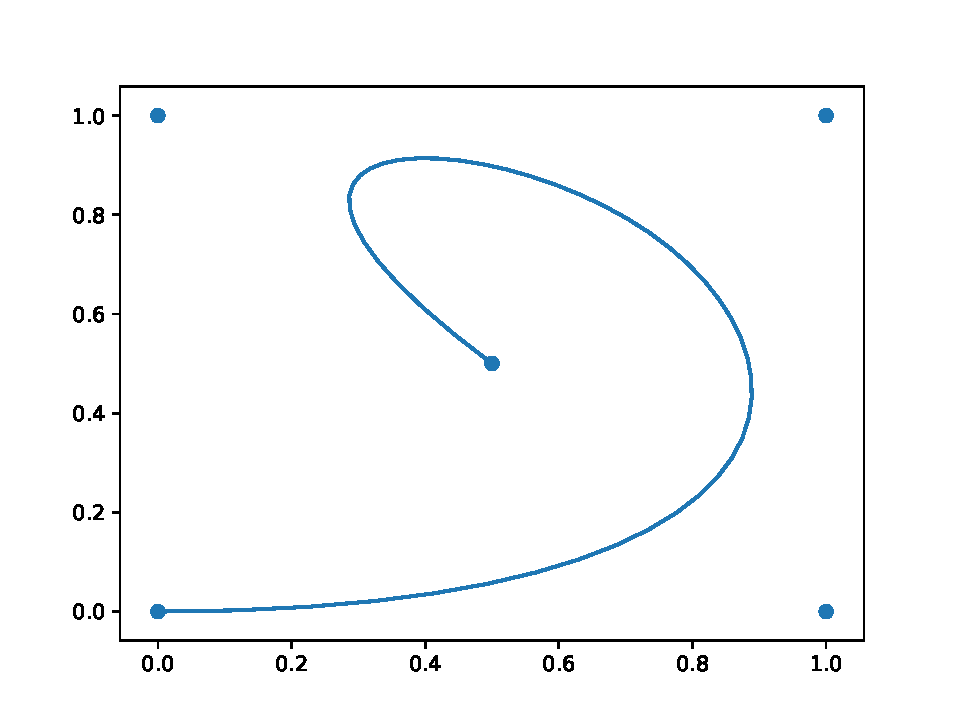
\includegraphics[width=\textwidth]{b_spline_curve.pdf}
\end{minipage}

\end{tabular}
\end{adjustbox}
\end{frame}

\begin{frame}{Multiskalenanalyse von Splinekurven}
Analyse von B-Spline-Kurven ergibt sich Komponentenweise.
\\[1.0cm]
Kochrezept:
\begin{itemize}
\item
Geschachtelte Splineräume: \\
Die Splineräume $V_d^k$ eines Grades $d$ zu den Knoten
\[
\mathbf{t}^k=(\frac{0}{2^k},\frac{1}{2^k},...,\frac{2^k-1}{2^k},\frac{2^k}{2^k})
\]
sind geschachtelt. Wähle als Skalenfunktionen die B-Splines zu
\[
\mathbf{\tau}^k=(\underbrace{0,...,0}_{d},\frac{0}{2^k},\frac{1}{2^k},...,\frac{2^k-1}{2^k},\frac{2^k}{2^k},\underbrace{1,...,1}_{d})
.
\]
\end{itemize}
\end{frame}


% Splitte Folie vermutlich etwa hier...

\begin{frame}{Multiskalenanalyse von Splinekurven}
\begin{itemize}
\item Standard-Skalarprodukt:
\[
\langle f,g\rangle =\int_0^1f(x)g(x)dx
\]
\item Wavelets:\\
Wahl ist nicht eindeutig! Man verlangt zum Beispiel minimalen Träger, um die Wavelets festzulegen. Diese beschleunigt zudem die Berechnungen.
\end{itemize}
\end{frame}

}




%\section{Anwendungen}
%	
%	{\setbeamertemplate{frame footer}{Quelle}
%	\begin{frame}{Titel}
%		\begin{columns}[T,onlytextwidth]
%			\column{0.75\textwidth}
%			Inhalt
%			\column{0.25\textwidth}
%			Inhalt 2
%		\end{columns}
%		Inhalt 3 \pause
%		\begin{columns}[c,onlytextwidth]
%			\column{0.38\textwidth}
%			\centering
%			Inhalt 4
%			
%			\column{0.61\textwidth}
%			\vspace{15pt}\ \\
%			\centering {\large$\Rightarrow$ Inhalt 5}
%		\end{columns}
%	\end{frame}}

	\appendix

	\begin{frame}[standout]
		Vielen Dank!	
	\end{frame}

	\blankframe
	
	
	
	
	
	
	
	
%	\begin{frame}[fragile]{Metropolis}
%		
%		The \themename theme is a Beamer theme with minimal visual noise
%		inspired by the \href{https://github.com/hsrmbeamertheme/hsrmbeamertheme}{\textsc{hsrm} Beamer
%			Theme} by Benjamin Weiss.
%		
%		Enable the theme by loading
%		
 %		\begin{verbatim}    \documentclass{beamer}
%		\usetheme{metropolis}\end{verbatim}
%		
%		Note, that you have to have Mozilla's \emph{Fira Sans} font and XeTeX
%		installed to enjoy this wonderful typography.
%	\end{frame}
%	\begin{frame}[fragile]{Sections}
%		Sections group slides of the same topic
%		
%		\begin{verbatim}    \section{Elements}\end{verbatim}
%		
%		for which \themename provides a nice progress indicator \ldots
%	\end{frame}
%	
%	\begin{frame}{Metropolis titleformats}
%		\themename supports 4 different titleformats:
%		\begin{itemize}
%			\item Regular
%			\item \textsc{Smallcaps}
%			\item \textsc{allsmallcaps}
%			\item ALLCAPS
%		\end{itemize}
%		They can either be set at once for every title type or individually.
%	\end{frame}
%	
%	{
%		\metroset{titleformat frame=smallcaps}
%		\begin{frame}{Small caps}
%			This frame uses the \texttt{smallcaps} titleformat.
%			
%			\begin{alertblock}{Potential Problems}
%				Be aware, that not every font supports small caps. If for example you typeset your presentation with pdfTeX and the Computer Modern Sans Serif font, every text in smallcaps will be typeset with the Computer Modern Serif font instead.
%			\end{alertblock}
%		\end{frame}
%	}
%	
%	{
%		\metroset{titleformat frame=allsmallcaps}
%		\begin{frame}{All small caps}
%			This frame uses the \texttt{allsmallcaps} titleformat.
%			
%			\begin{alertblock}{Potential problems}
%				As this titleformat also uses smallcaps you face the same problems as with the \texttt{smallcaps} titleformat. Additionally this format can cause some other problems. Please refer to the documentation if you consider using it.
%				
%				As a rule of thumb: Just use it for plaintext-only titles.
%			\end{alertblock}
%		\end{frame}
%	}
%	
%	{
%		\metroset{titleformat frame=allcaps}
%		\begin{frame}{All caps}
%			This frame uses the \texttt{allcaps} titleformat.
%			
%			\begin{alertblock}{Potential Problems}
%				This titleformat is not as problematic as the \texttt{allsmallcaps} format, but basically suffers from the same deficiencies. So please have a look at the documentation if you want to use it.
%			\end{alertblock}
%		\end{frame}
%	}
%	
%	\begin{frame}[fragile]{Typography}
%		\begin{verbatim}The theme provides sensible defaults to
%		\emph{emphasize} text, \alert{accent} parts
%		or show \textbf{bold} results.\end{verbatim}
%		
%		\begin{center}becomes\end{center}
%		
%		The theme provides sensible defaults to \emph{emphasize} text,
%		\alert{accent} parts or show \textbf{bold} results.
%	\end{frame}
%	
%	\begin{frame}{Font feature test}
%		\begin{itemize}
%			\item Regular
%			\item \textit{Italic}
%			\item \textsc{SmallCaps}
%			\item \textbf{Bold}
%			\item \textbf{\textit{Bold Italic}}
%			\item \textbf{\textsc{Bold SmallCaps}}
%			\item \texttt{Monospace}
%			\item \texttt{\textit{Monospace Italic}}
%			\item \texttt{\textbf{Monospace Bold}}
%			\item \texttt{\textbf{\textit{Monospace Bold Italic}}}
%		\end{itemize}
%	\end{frame}
%	
%	\begin{frame}{Lists}
%		\begin{columns}[T,onlytextwidth]
%			\column{0.33\textwidth}
%			Items
%			\begin{itemize}
%				\item Milk \item Eggs \item Potatos
%			\end{itemize}
%			
%			\column{0.33\textwidth}
%			Enumerations
%			\begin{enumerate}
%				\item First, \item Second and \item Last.
%			\end{enumerate}
%			
%			\column{0.33\textwidth}
%			Descriptions
%			\begin{description}
%				\item[PowerPoint] Meeh. \item[Beamer] Yeeeha.
%			\end{description}
%		\end{columns}
%	\end{frame}
%	\begin{frame}{Animation}
%		\begin{itemize}[<+- | alert@+>]
%			\item \alert<4>{This is\only<4>{ really} important}
%			\item Now this
%			\item And now this
%		\end{itemize}
%	\end{frame}
%	\begin{frame}{Figures}
%		\begin{figure}
%			\newcounter{density}
%			\setcounter{density}{20}
%			\begin{tikzpicture}
%			\def\couleur{alerted text.fg}
%			\path[coordinate] (0,0)  coordinate(A)
%			++( 90:5cm) coordinate(B)
%			++(0:5cm) coordinate(C)
%			++(-90:5cm) coordinate(D);
%			\draw[fill=\couleur!\thedensity] (A) -- (B) -- (C) --(D) -- cycle;
%			\foreach \x in {1,...,40}{%
%				\pgfmathsetcounter{density}{\thedensity+20}
%				\setcounter{density}{\thedensity}
%				\path[coordinate] coordinate(X) at (A){};
%				\path[coordinate] (A) -- (B) coordinate[pos=.10](A)
%				-- (C) coordinate[pos=.10](B)
%				-- (D) coordinate[pos=.10](C)
%				-- (X) coordinate[pos=.10](D);
%				\draw[fill=\couleur!\thedensity] (A)--(B)--(C)-- (D) -- cycle;
%			}
%			\end{tikzpicture}
%			\caption{Rotated square from
%				\href{http://www.texample.net/tikz/examples/rotated-polygons/}{texample.net}.}
%		\end{figure}
%	\end{frame}
%	\begin{frame}{Tables}
%		\begin{table}
%			\caption{Largest cities in the world (source: Wikipedia)}
%			\begin{tabular}{lr}
%				\toprule
%				City & Population\\
%				\midrule
%				Mexico City & 20,116,842\\
%				Shanghai & 19,210,000\\
%				Peking & 15,796,450\\
%				Istanbul & 14,160,467\\
%				\bottomrule
%			\end{tabular}
%		\end{table}
%	\end{frame}
%	\begin{frame}{Blocks}
%		Three different block environments are pre-defined and may be styled with an
%		optional background color.
%		
%		\begin{columns}[T,onlytextwidth]
%			\column{0.5\textwidth}
%			\begin{block}{Default}
%				Block content.
%			\end{block}
%			
%			\begin{alertblock}{Alert}
%				Block content.
%			\end{alertblock}
%			
%			\begin{exampleblock}{Example}
%				Block content.
%			\end{exampleblock}
%			
%			\column{0.5\textwidth}
%			
%			\metroset{block=fill}
%			
%			\begin{block}{Default}
%				Block content.
%			\end{block}
%			
%			\begin{alertblock}{Alert}
%				Block content.
%			\end{alertblock}
%			
%			\begin{exampleblock}{Example}
%				Block content.
%			\end{exampleblock}
%			
%		\end{columns}
%	\end{frame}
%	\begin{frame}{Math}
%		\begin{equation*}
%			e = \lim_{n\to \infty} \left(1 + \frac{1}{n}\right)^n
%		\end{equation*}
%	\end{frame}
%	\begin{frame}{Line plots}
%		\begin{figure}
%			\begin{tikzpicture}
%			\begin{axis}[
%			mlineplot,
%			width=0.9\textwidth,
%			height=6cm,
%			]
%			
%			\addplot {sin(deg(x))};
%			\addplot+[samples=100] {sin(deg(2*x))};
%			
%			\end{axis}
%			\end{tikzpicture}
%		\end{figure}
%	\end{frame}
%	\begin{frame}{Bar charts}
%		\begin{figure}
%			\begin{tikzpicture}
%			\begin{axis}[
%			mbarplot,
%			xlabel={Foo},
%			ylabel={Bar},
%			width=0.9\textwidth,
%			height=6cm,
%			]
%			
%			\addplot plot coordinates {(1, 20) (2, 25) (3, 22.4) (4, 12.4)};
%			\addplot plot coordinates {(1, 18) (2, 24) (3, 23.5) (4, 13.2)};
%			\addplot plot coordinates {(1, 10) (2, 19) (3, 25) (4, 15.2)};
%			
%			\legend{lorem, ipsum, dolor}
%			
%			\end{axis}
%			\end{tikzpicture}
%		\end{figure}
%	\end{frame}
%	\begin{frame}{Quotes}
%		\begin{quote}
%			Veni, Vidi, Vici
%		\end{quote}
%	\end{frame}
%	
%	{%
%		\setbeamertemplate{frame footer}{My custom footer}
%		\begin{frame}[fragile]{Frame footer}
%			\themename defines a custom beamer template to add a text to the footer. It can be set via
%			\begin{verbatim}\setbeamertemplate{frame footer}{My custom footer}\end{verbatim}
%		\end{frame}
%	}
%	
%	\begin{frame}{References}
%		Some references to showcase [allowframebreaks] \cite{knuth92,ConcreteMath,Simpson,Er01,greenwade93}
%	\end{frame}
%	
%	\begin{frame}{Summary}
%		
%		Get the source of this theme and the demo presentation from
%		
%		\begin{center}\url{github.com/matze/mtheme}\end{center}
%		
%		The theme \emph{itself} is licensed under a
%		\href{http://creativecommons.org/licenses/by-sa/4.0/}{Creative Commons
%			Attribution-ShareAlike 4.0 International License}.
%		
%		\begin{center}\ccbysa\end{center}
%		
%	\end{frame}
%	
%	\begin{frame}[standout]
%		Questions?
%	\end{frame}
%	
%	\appendix
%	
%	\begin{frame}[fragile]{Backup slides}
%		Sometimes, it is useful to add slides at the end of your presentation to
%		refer to during audience questions.
%		
%		The best way to do this is to include the \verb|appendixnumberbeamer|
%		package in your preamble and call \verb|\appendix| before your backup slides.
%		
%		\themename will automatically turn off slide numbering and progress bars for
%		slides in the appendix.
%	\end{frame}
%	
%	\begin{frame}[allowframebreaks]{References}
%		
%		\bibliography{demo}
%		\bibliographystyle{abbrv}
%		
%	\end{frame}
	
\end{document}
